\section{Clustering\label{cluster}}
A metric for article relevance was sought, and traditional nearest
neighbour algorithms formed the basis for this measure.  Using $k$-NN
approaches for small numbers of query documents yields $k$ documents
ranked by their cosine similarity to a given document.  The cosine
similarity refers to angular distance between the two documents
plotted in a vector space (Section \ref{vecs}).  There are many ways
to place documents in a vector space.  As discussed in Section
\ref{vecs}, a {\it state of the art} solution trains document vectors
on a large document corpus.  This has drawbacks, however, since
it relies on knowing the documents that are being clustered in
advance, and results from the algorithm are only available at the
end of execution time (several hours).  In
other words, the state of the art is not an {\it online}
algorithm.

\nr{} uses pre-trained word-level vectors to
produce document vectors on the fly.  This way,
a document vector can be calculated using only the document and
the static set of word vectors.
Each word in the document forms a piece of
a weighted aggregate vector.  Words nearer to the beginning of the
document play a stronger role in the overall document vector than
words closer to the end.  This dampening was achieved using
survival function formulae.  The motivation for using these formulae
comes intuitively from the notion of reader attention.  The model
assumes most readers don't {\it survive} to the end of the document,
and that documents contain more important information nearer to top.
These word vectors are referred to as {\it weak document vectors}
to distinguish them from higher quality word vectors
bulk-produced using strong neural networks.

The efficacy of the weak document vectors were tested by applying
them as the singular feature source in AdaBoost document
classification.  Although the resulting F1 scores were lower than
when all feature sources were used, the score was still
sufficiently high (roughly 75\% on the test set) to determine that
semantic meaning was present in the weak document vectors.
\begin{figure}[H]
    \centering
    \fbox{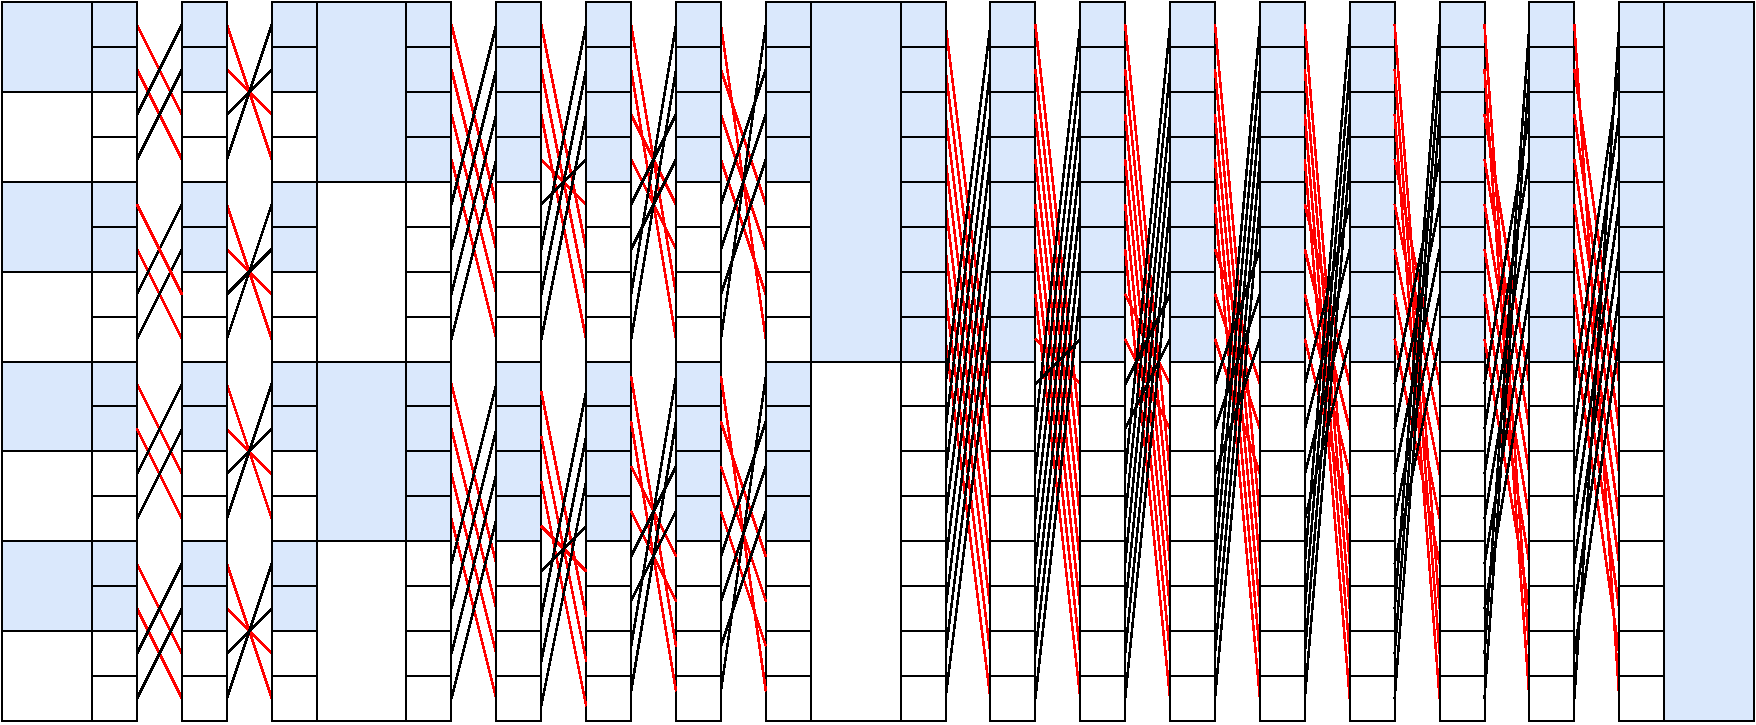
\includegraphics[width=0.8\textwidth]{media/similarities.pdf}}
    \caption{
        \raggedright
        An illustration of the parallel execution pattern used in bulk nearest neighbour
        processing.\label{simi}
    }
\end{figure}
These document vectors could then be used in order to cluster documents
together by cosine similarity.  Rather than finding $k$ nearest
neighbours to a given document or small set of documents, a heavier
task was undertaken, determining similarity scores across all news
resource pairs crawled in a set time period.  A naive solution,
when applied to 1,000,000 vectors, would take roughly 57 hours
to complete, longer than a news cycle.  This naive approach would
iterate through the cartesian product of the dataset, and find the
similarity score for each tuple pair.

An improvement would be to split the dataset into $P$ chunks
(where $P$ is the number of processor cores available),
and calculate the similarity for all possible tuple pairs in the
chunk.  After this first stage, each chunk would be left
{\it calculated}, i.e. the similarity between each tuple pair from the
chunk would be known. All cores would be used in the initial production
of $P$ chunks, but in subsequent steps,
when similarities across disparate chunks are sought,
the core utilisation would decrease.  In the final stage, when two
large chunks are being merged, only one core would be used.
This problem is comparable to the diminishing returns observed in
parallel implementations of divide-and-conquer sorting algorithms
(merge sort and quick sort).

\nr{} uses a bulk nearest neighbour algorithm that ensures all
cores are being used at all stages of execution.  The formal
foundation of the algorithm is divide and conquer.  Figure \ref{simi}
attempts to illustrate the algorithm's execution.  Two chunks are
{\it merged} into one chunk by splitting chunks $A$ and
$B$ into equal {\it subparts}, and calculating the similarities
between items from each combination of subparts from $A$ and $B$.
Red lines signify the process of {\it merging} two chunks.  Merging
effictively turns two chunks into one chunk, where the previously
mentioned {\it calculated} property holds true.
The black lines are present only to illustrate the reflexive nature
of calculating similarity; the cosine similarity between
vectors $V$ and $U$ is the same as the cosine similarity between
vectors $U$ and $V$.